\documentclass[a4paper, 12pt]{article}
\usepackage[utf8]{inputenc}
\DeclareUnicodeCharacter{2074}{\ensuremath{{}^4}}
\usepackage{listings}
\usepackage{graphicx}
\title{Obligatorisk innlevering 2}
\author{Sivert M. Skarning}
\date{Mai 2019}
\begin{document}
\maketitle

\section{Oppgave 1}
\subsection{Oppgavebeskrivelse}
Implementere DFT og IDFT på egen hånd. Algoritmene skal implementeres slik som gitt i boka, hvis ikke annet er tydelig dokumentert i egen rapport. Algoritmenes korrekthet skal demonstreres på enkle bilder.

\subsection{Dokumentasjon}
I oppgave 1 har jeg laget et skript som tar inn et valgt bilde og fouriertransformerer og invers-fouriertransformerer et bilde både med innebygde funksjoner og med egenskrevne funksjoner. De egenskrevne funksjonene er har en effektivitet på $O(n⁴)$. De er følgelig veldig trege for de store bildene. Dette gjør at bildene jeg har brukt er veldig små.
\subsection{Resultat}
Som et eksempel bilde valgte jeg en 30x30 bilde av et rektangel. For å teste at implementasjonen mine fungerer, bruker jeg fft pack sine funkjsoner for å gjøre samme transformasjon. Man ser følgelig at figur \ref{fig:fft} er lik \ref{fig:dft} og at figur \ref{fig:ifft} er lik \ref{fig:idft}. Dette vil si at implementasjonen skal fungere. Vist man observerer figur \ref{fig:dft} ser vi at det er to retninger som dominerer. Den sterkeste retningen er den horisontale retningen. Fordi oppløsningen er så dårlig ser vi at det vil danne seg overgagner i intensitet på det spatiale bilde i vertikal retning. Det er derfor vi får flere linjer i horisontal retning i det fouriertransformerte bilde.

\section{Oppgave 2}
\subsection{oppgavebeskrivelse}
Utfør skjærping og utjevning i både frekvens- og spatial-domenet på Lena og Barbara. Resultatene skal dokumenteres og sammenlignes i rapporten. Det er lov å bruke innebygde operatorer, men filterne skal lages manuelt.
\subsection{Dokumentasjon}
I denne oppgaven valgte jeg å bruke to typer filtere i frekvensdomenet.
\begin{itemize}
\item Lowpass Ideal-filter
\item Highpass Ideal-filter
\end{itemize}

Jeg valgte også to filtere i det spatiale domenet

\begin{itemize}
\item Gaussian blure
\item Laplacian sharpening
\end{itemize}

Disse filterne er lette å implemetere i frekvensdomenet. Når bilde er konvertert med fast fourier transformasjon trenger man kun å gange filteret med bilde for å få til en konvolusjon. For å lage filteret lagde jeg en funksjon som finner lengde fra senter til et gitt pixel. Ved hjelp av denne funksjonen velger jeg en radius hvor alle frekvensene utenfor denne radiusen blir fjernet. Jeg prøvde cut-off frekvens på 30 og på 90.
\subsection{Resultat}
Til venstre i  figur \ref{fig:bgl} ser du barbara filterert med gaussian blure med standardavvik på 5 og til høyre ser du barbara filtrert med et lavpass filter med cut-off frekvens på 30.

I figur \ref{fig:lhl} ser du lena filterert med et høypass filter med cut-off frekvens på 30, til venstre ser du barbara filteret med et laplacian filter.

 Ved å se på figur \ref{fig:bgl} kan vi se at et gaussisk filter gir mindre støy på bilde og en jevnere blure. Det gussiks filtere er dermed ikke like bra til å bevare kantene på bilde. I figur \ref{fig:ihl} ser vi at høypass filteret er kraftigere enn laplacian filteret. Dette kan endres ved å sette cut off frekvensen til en laver verdi.


\begin{figure}[h]
  \centering
  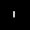
\includegraphics[width=0.5\textwidth]{images/rektangel.png}
  \caption{Rektangel i spatialt domene}
  \label{fig:rektangel}
\end{figure}


\begin{figure}[h]
  \centering
  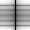
\includegraphics[width=0.5\textwidth]{images/fftpack-rektangel}
  \caption{Rektangel i frekvensdomene, FFT pack}
  \label{fig:fft}
\end{figure}


\begin{figure}[h]
  \centering
  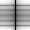
\includegraphics[width=0.5\textwidth]{images/myfft-rektangel}
  \caption{Rektangel i frekvensdomene, egenimplementert dft funksjon}
  \label{fig:dft}
\end{figure}


\begin{figure}[h]
  \centering
  
\includegraphics[width=0.5\textwidth]{images/ifft-rektangel}
  \caption{Rektangel i det spatiale domene(ifft)}
  \label{fig:ifft}
\end{figure}


\begin{figure}[h]
  \centering
  
\includegraphics[width=0.5\textwidth]{images/idft-rektangel}
  \caption{Rektangel i det spatiale domene, egenimplementert idft funksjon}
  \label{fig:idft}
\end{figure}


\begin{figure}[h]
  \centering
  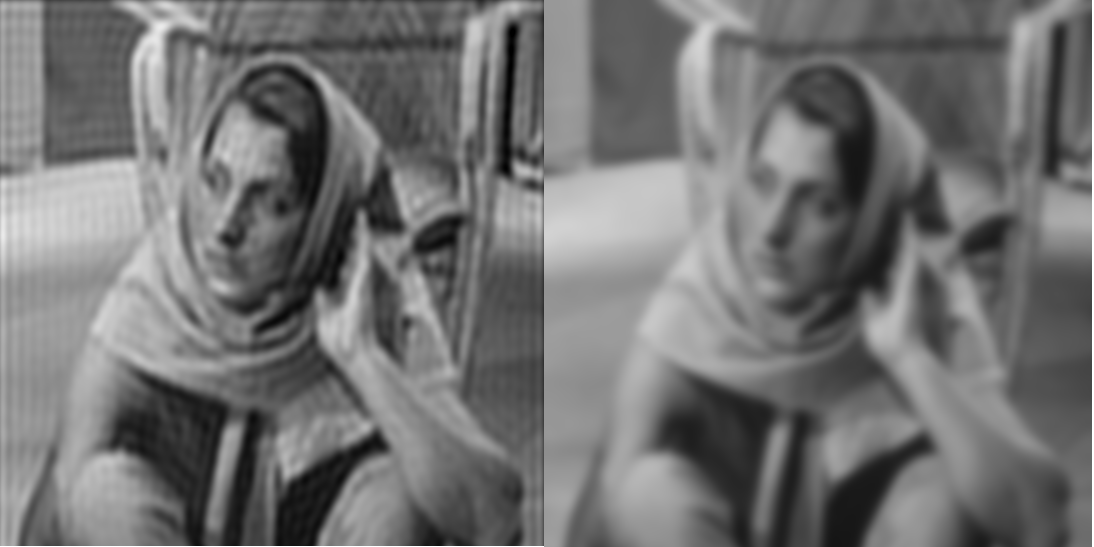
\includegraphics[width=0.8\textwidth]{images/barbara-gaussian-lowpass.png}
  \caption{Gaussian blure(5) og lowpass(30)}
  \label{fig:bgl}
\end{figure}


\begin{figure}[h]
  \centering
  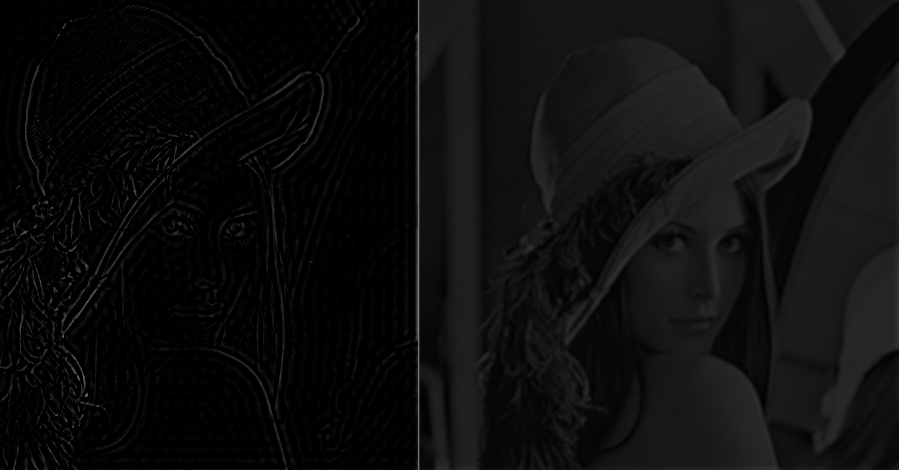
\includegraphics[width=0.8\textwidth]{images/lena-highpass-laplacian.png}
  \caption{Higpass(30) og Laplacian}
  \label{fig:lhl}
\end{figure}
\end{document}